\documentclass[handout]{beamer}

\usepackage[utf8]{inputenc} % Language and font encoding
\usepackage[icelandic]{babel}
\usepackage[T1]{fontenc}


\usepackage{tikz}
\usepackage[listings,theorems]{tcolorbox}
\usepackage{booktabs}
\usepackage{minted} %Minted and configuration
\usemintedstyle{default}

\renewcommand{\theFancyVerbLine}{\sffamily \arabic{FancyVerbLine}}
%%%%%%%%%%%
% More math
%%%%%%%%%%%
\newcommand{\Mod}[1]{\ \text{mod}\ #1}

%%%%%%%%%%%%%%%%%%%%%%
% Beamer configuration
%%%%%%%%%%%%%%%%%%%%%%
\setbeamertemplate{navigation symbols}{}
\usecolortheme{dove}
\setbeamercolor{frametitle}{fg=white}

\usebackgroundtemplate%
{%
\vbox to \paperheight{

\includegraphics[width=\paperwidth]{Pics/hi-slide-head-2016}

\vfill
\hspace{0.5cm}
\includegraphics[width=0.3\paperwidth]{Pics/hi-von-logo}
\vspace{0.4cm}
    }%
}

\AtBeginSection[]
{
  \begin{frame}<beamer>
    \frametitle{Yfirlit}
    \tableofcontents[currentsection]
  \end{frame}
}

\setbeamerfont{frametitle}{size=\normalsize}
\addtobeamertemplate{frametitle}{}{\vspace*{0.5cm}}

%%%%%%%%%%%%%%%%%%%%%%%%%
% tcolorbox configuration
%%%%%%%%%%%%%%%%%%%%%%%%%

% Setup from: http://tex.stackexchange.com/a/43329/21638
\tcbset{%
    noparskip,
    colback=gray!10, %background color of the box
    colframe=gray!40, %color of frame and title background
    coltext=black, %color of body text
    coltitle=black, %color of title text 
    fonttitle=\bfseries,
    alerted/.style={coltitle=red, colframe=gray!40},
    example/.style={coltitle=black, colframe=green!20, colback=green!5},
}


%%%%%%%%%%%%%%%%%%%%%%%
% Further configuration
%%%%%%%%%%%%%%%%%%%%%%%
\hypersetup{colorlinks=true,pdfauthor={Eirikur Ernir Thorsteinsson},linkcolor=blue,urlcolor=blue}
\graphicspath{{./Pics/}}

\author{Eiríkur Ernir Þorsteinsson}
\institute{Háskóli Íslands}
\date{Haust 2016}

\title{Stærðfræðimynstur í tölvunarfræði}
\subtitle{Vika 6, seinni fyrirlestur}

\begin{document}

\begin{frame}
\titlepage
\end{frame}


\section{Inngangur}

\begin{frame}{Í síðasta tíma}
\begin{itemize}
 \item Upprifjun á rakningarvenslum
 \item Endurkvæm reiknirit
\end{itemize}
\end{frame}

\begin{frame}{Af hverju virkar þrepun?}
\begin{itemize}
 \item Þrepun er ekki göldrótt!
 \item Í hefðbundnu grunnskrefi þrepunarsönnunar sýnum við að staðhæfing $P(1)$ sé sönn
 \item Í þrepunarskrefi þrepunarsönnunar sýnum við fram á að $P(k) \to P(k+1)$ fyrir ótilgreinda heiltölu $k$
 \item Þá getum við séð fyrir okkur að $P(n)$ gildi fyrir allar jákvæðar heiltölur $n$
 \begin{itemize}
  \item Af hverju?
  \item $P(1)$ er satt og við vitum að ef $P(1)$ er satt þá er $P(2)$ líka satt
  \item Þá er $P(2)$ satt og við vitum að ef $P(2)$ er satt þá er $P(3)$ líka satt\ldots
  \item Sönnun í bók
 \end{itemize}
\end{itemize}
\end{frame}

\section{Endurkvæm reiknirit}

\begin{frame}{Endurkvæm reiknirit}
\begin{itemize}
 \item Munum að reiknirit er endanleg runa vel skilgreindra aðgerða sem reikna út lausn á skilgreindu vandamáli
 \item Reiknirit hefur inntak, sem lýsir tilviki af vandamálinu sem það leysir
 \item Reiknirit er kallað endurkvæmt ef það leysir vandamálið með því að smætta það niður í smærra tilvik af sama vandamáli
\end{itemize}
\end{frame}

\begin{frame}{Endurkvæmt hrópmerkt}
Hrópmerkt hentar vel til endurkvæms útreiknings.
\begin{center}
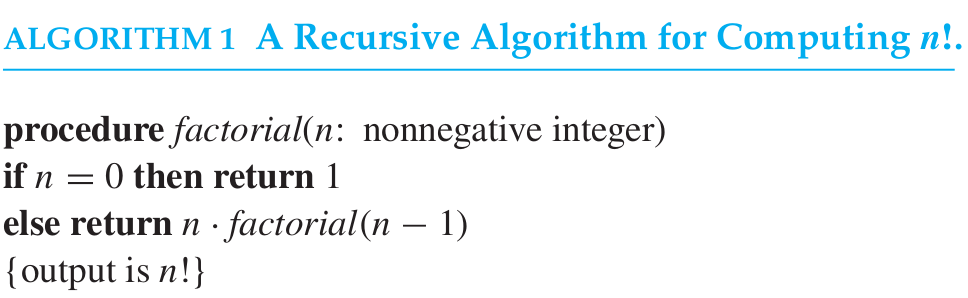
\includegraphics[width=\textwidth]{factorial-algorithm}
\end{center}
\[
3! = 3\cdot 2! = 3 \cdot 2 \cdot 1! = 3 \cdot 2 \cdot 1
\]
\end{frame}

\begin{frame}{Endurkvæmt GCD}
\begin{columns}
\column{0.5\textwidth}
Við getum reiknað stærsta samdeili (gcd) með endurkvæmu reikniriti sem byggir á því að 
\[
 gcd(a,b) = gcd(b \Mod a, a)
\]
og að 
\[
 gcd(0,b) = b
\]
þegar $b > 0$.
\column{0.5\textwidth}
Þannig getum við reiknað stærsta samdeili 5 og 8:
\begin{align*}
gcd(5,8) &= gcd(8 \Mod 5, 5)\\
&= gcd(3,5)\\
&= gcd(5 \Mod 3, 3)\\
&= gcd(2,3)\\
&= gcd(3 \Mod 2, 2)\\
&= gcd(1,2)\\
&= gcd(2 \Mod 1, 1)\\
&= gcd(0,1)\\
&= 1
\end{align*}

\end{columns}
\end{frame}



\begin{frame}{Næst}
???
\end{frame}


\end{document}
